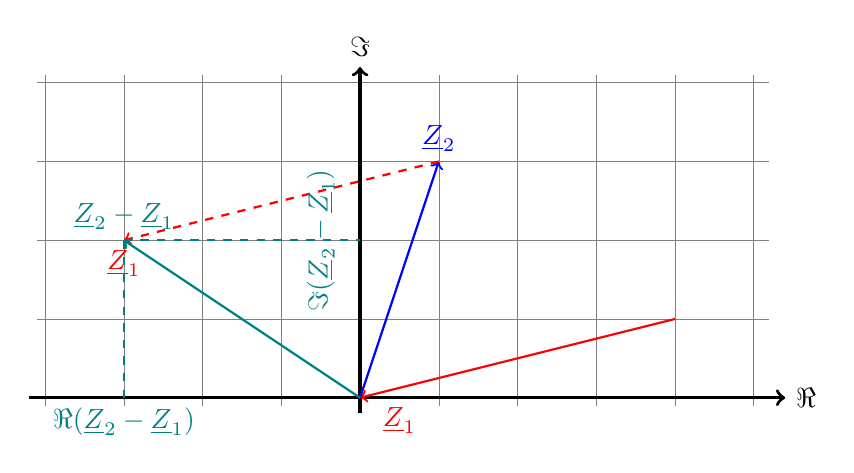
\begin{tikzpicture}
    \draw (0,0) coordinate (K);
    \draw[very thin,gray] (-4.1,-0.1) grid (5.2,4.1);
    \draw[->, very thick] (-4.2,0) -- (5.4,0) node[right] {$\Re$};
    \draw[->, very thick] (0,-0.2) -- (0,4.2) node[above] {$\Im$};
    \draw[->, thick, red] (4,1) -- (0,0);
    \draw(0.5,0) node [below,red] {$\underline{Z}_\mathrm{1}$};
    \draw[->, thick, blue] (0,0) -- (1,3) node[above] {$\underline{Z}_\mathrm{2}$};
    \pause

    \draw[->, dashed, thick, red] (1,3) -- (-3,2) node[left, below] {$\underline{Z}_\mathrm{1}$};
    \pause

    \draw[->, thick, teal] (0,0) -- (-3,2) node [teal, above] {$\underline{Z}_\mathrm{2}-\underline{Z}_\mathrm{1}$};
    \draw[dashed, thick, teal] (-3,2) -- (0,2)
    (-0.5,2) node[rotate=90] {$\Im(\underline{Z}_\mathrm{2}-\underline{Z}_\mathrm{1}$)};
    \draw[dashed, thick, teal] (-3,2) -- (-3,0) node[below] {$\Re(\underline{Z}_\mathrm{2}-\underline{Z}_\mathrm{1}$)};
\end{tikzpicture}